%LLPStartPreview para rodar o pdf com mudancas automaticas


\documentclass{article}
\usepackage{graphicx}
\usepackage{wrapfig}
\usepackage[utf8]{inputenc}
\usepackage[brazil]{babel} % Separacao de silabas em portugues
\usepackage{amsthm} % has proof
\usepackage{listings}



\renewcommand\refname{Referências}
\newtheorem{theorem}{Teorema}[section]
\newtheorem{corollary}{Corolário}
\newtheorem{lemma}{Lema}

\title{O problema do carteiro chinês}
\date{}

\begin{document}

\maketitle

\section{As sete pontes de Königsberg}

O problema das sete pontes de Königsberg foi descrito e solucionado pelo matemático Leonhard Euler em 1736, o problema consistia em decidir se seria possível traçar no mapa de Königsberg um trajeto que percorresse cada uma de suas 7 pontes uma única vez, sem repetições.

A importância deste problema é enorme para a área da computação, já que o artigo de Euler publicado sobre ele é considerado o primeiro artigo sobre teoria dos grafos.

\begin{wrapfigure}{r}{0.5\textwidth} 
    \centering
    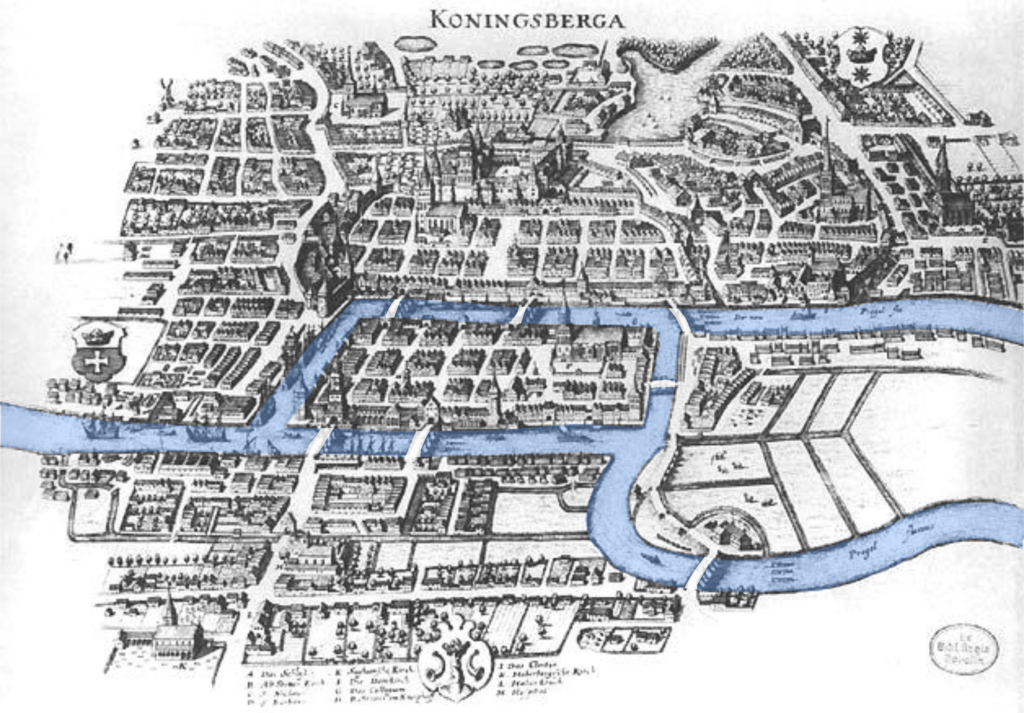
\includegraphics[width=0.5\textwidth]{konigsberg.png}
    \caption{Representação das sete pontes de Königsberg}
\end{wrapfigure}

Vamos definir como \textbf{passeio} em um grafo uma sequência finita não vazia $P = \{ v_0, a_1, v_2, a_2, \dots, a_k, v_k\}$, cujos termos são alternadamente vértices $v_i$ e arestas $a_j$ e tal que, para todo $i$, $1 \leq i \leq k$, os extremos de $a_i$ são $v_{i-1}$ e $v_i$. 
Os vértices $v_0$ e $v_k$ são a origem e o término de $P$, respectivamente; e os vértices $v_1, v_2, \dots, v_{k-1}$ são chamaos vértices internos de P. 

Uma \textbf{trilha} é um passeio sem arestas repetidas. 
Um \textbf{caminho} é um passeio sem vértices repetidos.
Por comprimento de um passeio, denotado por $||P||$, é o número de arestas de $P$.

Um passeio é considerado \textbf{fechado} se sua origem e término são iguais.

Uma trilha fechada cuja origem e vértices internos são todos distintos é um \textbf{circuito}.

Devido às contribuições de Euler ao problema descrito, definiu-se \textbf{trilha euleriana} (ou caminho euleriano) como uma trilha que passa por todas arestas de um grafo e \textbf{grafo euleriano} como um grafo que possui uma trilha euleriana fechada (também chamado de circuito euleriano).

Euler modelou essa área da cidade como um grafo, representado na figura \ref{konigsberg-graph}, tratando as pontes como arestas e as massas de terra como vértices.
A partir de tal modelagem e das definições feitas, o problema de Königsberg consiste, em definir se o grafo que representa a cidade possui ou não uma trilha euleriana. 


\begin{wrapfigure}{l}{0.25\textwidth}
    \centering
    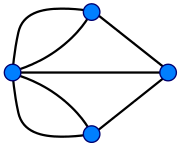
\includegraphics[width=0.25\textwidth]{konigsberg-graph.png}
    \caption{Modelagem de Königsberg como um grafo}
    \label{konigsberg-graph}
\end{wrapfigure}

O matemático provou que uma condição necessária para que um grafo seja euleriano é que todos seus vértices possuam grau par; 
ele também afirmou, porém sem prova, que qualquer grafo conexo cujos vértices possuem grau par é euleriano.

A prova para essa afirmação só foi publicada mais de cem anos depois, em 1873, por Carl Hierholzer \cite{hierholzer}.

\begin{theorem}[Teorema de Euler ou de Euler-Hierholzer]
    \label{euler}
    Um grafo é euleriano se, e somente se, é conexo e todos seus vértices possuem grau par.
\end{theorem}

Antes de trabalhar na prova de tal teorema, primeiramente trabalharemos em um lema:

\begin{lemma}
	Se $G$ é um grafo tal que todos seus vértices possuem grau maior ou igual a 2, então $G$ possui um ciclo.
\end{lemma}

\begin{proof}
	Vamos assumir que um grafo qualquer $G = \{V, A\}$ não possui um ciclo, neste caso $G$ deverá possuir no máximo $|V| - 1$ arestas, havendo assim a possibilidade de $G$ ser uma árvore. 
	
	Como cada aresta contribui em duas unidades para a soma dos graus de um grafo, se vale que $|A| \leq |V|-1$ então vale também que $\sum_{v \in V} g(v) \leq 2|V| - 2$, sendo $g(u)$ o grau de um vértice $u$. 

	Porém, faz parte da hipótese do lema que todos vértices possuem grau maior ou igual a 2, o que implica na seguinte desigualdade: $\sum_{v \in V}g(v) \geq 2|V|$, o que é inconsistente com o que havíamos descoberto.
	
	Por contradição, provamos que $G$ deverá possuir ciclos dadas as condições do lema.
\end{proof}

% TODO: o que é um ciclo?

Provado tal lema, podemos agora provar o teorema \ref{euler}:

\begin{proof}

Seja $G = \{V, E\}$ o grafo em questão.

Começamos provando que se um grafo é euleriano e conexo então todos seus vértices possuem grau par.

Seja $T$ uma trilha euleriana fechada, cuja existência é garantida já que $G$ é euleriano. Cada vez que um vértice $v$ ocorre em $T$ ela é precedida de uma aresta que liga um vértice qualquer a $v$ e sucedida de outra aresta ligando $v$ a um vértice qualquer. 
Um caso especial é quando o vértice $v$ em questão é a origem (e o término) de $T$: neste caso a aresta que o precede é a última aresta presente em $T$, e a aresta que o sucede é a primeira aresta da trilha.


Agora, provaremos por indução no número de arestas de $G$ que se $G$ for conexo e se todos seus nós possuem grau par, então ele é euleriano.

% Como tratar o caso de varios vertices de grau zero no grafo? O grafo nao é conexo, mas pode ser euleriano

\end{proof}

\begin{corollary}
    Um grafo possui um caminho euleriano se, e somente se, é conexo e possui apenas zero ou dois vértices de grau ímpar.
\end{corollary}

\begin{proof}
    Seja $G$ um grafo conexo qualquer. Realizaremos a demonstração para os seguintes casos:
    \begin{enumerate}
        \item $G$ não possui vértices de grau ímpar. Neste caso, $G$ possui, segundo o teorema \ref{euler}, um circuito euleriano, que é um tipo de caminho euleriano.
        
        \item $G$ possui apenas um vértice de grau ímpar. Este caso é impossível de se acontecer, já que a soma do grau de todos vértices deve ser par.
        
        \item $G$ possui dois vértices de grau ímpar. 
        Sejam $u$ e $v$ os únicos vértices de $G$ que possuem grau ímpar.
        Adiciona-se uma aresta fictícia ao grafo $G$, a aresta $uv$, fazendo com que tanto $u$ quanto $v$ possuam graus pares. 
		Chamaremos o grafo $G$ acrescido da aresta $uv$ de $G'$.
        Como $u$ e $v$ eram os únicos vértices de grau ímpar de $G$, vale que todos vértices de $G'$ possuirão grau par. 
		Além disso, vale que $G'$ é conexo, pois faz parte da premissa que o grafo original $G$ era conexo.

        Sendo assim, podemos aplicar o teorema \ref{euler}, provando a existência de um circuito euleriano em $G'$, que chamaremos de $C$.
        Como $C$ é um circuito euleriano, isso implica que $uv \in C$.

        \item $G$ possui três ou mais vértices de grau ímpar.
    \end{enumerate}
\end{proof}


Como os quatro vértices do grafo da figura \ref{konigsberg-graph} possuem grau ímpar, é impossível, pela condição estabelecida, que exista um caminho euleriano.


Segue agora uma implementação de um algoritmo que encontra o circuito euleriano de um grafo dado que o mesmo possui um circuito euleriano:


 
\lstinputlisting[language=c++]{euler_cycle.cpp}
\section{Undirected CPP}

O grafo deverá ser conexo.
\\

\textbf{Solução:} 
\begin{enumerate}
    \item Criar um grafo completo ligando todos vértices $u, v$ que possuirem grau ímpar com arestas de custo igual ao menor caminho entre $u$ e $v$. 
    \item Rodar algoritmo de emparelhamento perfeito de custo mínimo (Húngaro com otimização do Edmonds e Karp, $\mathcal{O}(n^3)$).
\end{enumerate}


\textbf{Observações:}
\begin{itemize}
		\item Pelo ``Lema do aperto de mão'' é garantido que haverá um número par de vértices de grau ímpar.
		\item Essa solução não se aproveita do grafo ser esparso, há outra formulação do Edmonds e Johnson que leva isso em consideração.
		\item Um problema similar é o de cobrir todas arestas com ciclos simples, de modo que o comprimento total dos ciclos é minimizado. Para grafos planares esses problemas são equivalentes.
	\end{itemize}

	\section{Directed CPP}

	O grafo deverá ser fortemente conexo.\\

	\textbf{Solução:}
	\begin{enumerate}
		\item Criar um grafo $P, Q$-bipartido completo. $P$ deve conter todos os vértices do grafo original com excesso de grau de entrada, e $Q$ deve conter todos vértices com excesso de grau de saída. que possuem valores diferentes de grau de entrada e saída. O custo das arestas entre $P$ e $Q$ deverá ser igual ao custo do menor caminho entre os dois vértices que a mesma liga.
		\item Modelar uma rede de fluxo: vértices de $P$ recebem um excesso igual a diferença do grau de entrada pelo grau de saída, vértices de $Q$ recebem uma demanda igual a diferença do grau de saída pelo grau de entrada. 
		\item Rodar um algoritmo de fluxo de custo mínimo. 
	\end{enumerate}

	\textbf{Observações:}
	\begin{itemize}
		\item Modelagem de fluxo com arestas de capacidade unitária, aumentando a velocidade do algoritmo.
	\end{itemize}

	\section{Mixed CPP}

	NP-hard, mesmo se $G$ for planar e se todos $c_{ij}$ forem iguais.

	\section{Windy Postman Problem}

	NP-hard

	Se todo ciclo do grafo tem o mesmo custo em ambos sentidos, transforma a aresta entre $i$ e $j$ de custos $c_{ij}$ e $c_{ji}$ em uma aresta não direcionada com custo $\frac{c_{ij} + c_{ji}}{2}$. Essa transformação reduz o problema de a um CPP não direcionado, que tem solução polinomial, porém para isso é necessário checar se todo ciclo tem o mesmo custo nas duas direções.

	\section{Hierarchical Postman Problem}

	NP-hard 

	Seja $P = \{A_1, A_2, \dots, A_k\}$ uma partição do conjunto de arestas $A$. Determinar um caminho em $G$ de custo mínimo que sai de um vértice $s$ e atinge um vértice $t$, respeitando uma hierarquia das arestas. O caminho só poderá possuir uma aresta pertencente a $A_j$ se o caminho passar anteriormente por todas arestas pertencentes a $A_i$, se $i < j$.


	\section{Anotações}

	\begin{itemize}
		\item Todo mixed CPP pode ser transformado em um WPP.
	\end{itemize}

	\medskip

	\begin{thebibliography}{9}
	\bibitem{konigsberg} 
	Euler, Leonhard
	\textit{Solution problematis ad geometriam situs pertinentis}. 
	Comment. Acad. Sci. U. Petrop 8, 128–40, 1736.

	\bibitem{hierholzer}
	Hierholzer, Carl
	\textit{``Über die Möglichkeit, einen Linienzug ohne Wiederholung und ohne Unterbrechung zu umfahren''}, 
	Mathematische Annalen, 6 (1): 30–32, doi:10.1007/BF01442866, 1873.
	\end{thebibliography}
 
\end{document}

\end{document}
